% 12pt: grandezza carattere
% a4paper: formato a4
% openright: apre i capitoli a destra
% twoside: serve per fare un
% documento fronteretro
% report: stile tesi (oppure book)
\documentclass[12pt,a4paper,openright,twoside]{report}

%libreria per scrivere in italiano
\usepackage[italian]{babel}

% libreria per accettare i caratteri
% digitati da tastiera come ?
% si può usare anche
% \usepackage[T1]{fontenc}
% però con questa libreria
% il tempo di compilazione
% aumenta
\usepackage[latin1]{inputenc}

% libreria per impostare il documento
\usepackage{fancyhdr}

% libreria per avere l'indentazione all'inizio dei capitoli, ...
\usepackage{indentfirst}

%libreria per mostrare le etichette
%\usepackage{showkeys}

% libreria per inserire grafici
\usepackage{graphicx}

% libreria per utilizzare font particolari ad esempio \textsc{}
\usepackage{newlfont}

% librerie matematiche
\usepackage{amssymb}
\usepackage{amsmath}
\usepackage{latexsym}
\usepackage{amsthm}

% librerie per mostrare il codice sorgente
\usepackage{listings, xcolor}
\renewcommand{\lstlistingname}{Codice sorgente}
\renewcommand{\lstlistlistingname}{Codici sorgenti}
% impostano i margini
\oddsidemargin=30pt
\evensidemargin=20pt

% serve per la sillabazione: tra parentesi vanno inserite come nell'esempio le parole
% che latex non riesce a tagliare nel modo giusto andando a capo.
\hyphenation{sil-la-ba-zio-ne pa-ren-te-si}

% comandi per l'impostazione della pagina, vedi il manuale della libreria fancyhdr per ulteriori delucidazioni
\pagestyle{fancy}\addtolength{\headwidth}{20pt}
\renewcommand{\chaptermark}[1]{\markboth{\thechapter.\ #1}{}}
\renewcommand{\sectionmark}[1]{\markright{\thesection \ #1}{}}
\rhead[\fancyplain{}{\bfseries\leftmark}]{\fancyplain{}{\bfseries\thepage}}
\cfoot{}

%comando per impostare l'interlinea
\linespread{1.3}

\begin{document}

\begin{titlepage}
% crea un ambiente libero da vincoli di margini e grandezza caratteri: si pu\`o modificare
% quello che si vuole, tanto fuori da questo ambiente tutto viene ristabilito

% elimina il numero della pagina
\thispagestyle{empty}

% imposta il margina superiore a 6.5cm
\topmargin=6.5cm

% incolonna la scrittura a destra
\raggedleft

% aumenta la grandezza del carattere a 14pt
\large

% emfatizza (corsivo) il carattere
\em

%\ldots lascia tre puntini
%\ldots

% va in una pagina nuova
\newpage

% non numera l'ultima pagina sinistra
\clearpage{\pagestyle{empty}\cleardoublepage}
\end{titlepage}

\pagenumbering{roman} % serve per mettere i numeri romani
\chapter*{Introduzione} % crea l'introduzione (un capitolo non numerato)

% imposta l'intestazione di pagina
\rhead[\fancyplain{}{\bfseries INTRODUZIONE}]{\fancyplain{}{\bfseries\thepage}}
\lhead[\fancyplain{}{\bfseries\thepage}]{\fancyplain{}{\bfseries INTRODUZIONE}}

% aggiunge la voce Introduzione nell'indice
\addcontentsline{toc}{chapter}{Introduzione}
% \ldots
Questo lavoro ha l'obiettivo di implementare sul simulatore Alchemist il modello Spatial Tuples.

Alchemist \`e un meta-simulatore estendibile, ispirato alla chimica stocastica e adatto al calcolo pervasivo e ai sistemi distribuiti. Fornisce un meta-modello flessibile, sul quale gli sviluppatori legano le proprie astrazioni, realizzando un'incarnazione.

Per creare l'incarnazione sar\`a necessario definire una base del modello ad agenti sul quale poi innestare Spatial Tuples.

% non numera l'ultima pagina sinistra
\clearpage{\pagestyle{empty}\cleardoublepage}

%crea l'indice
\tableofcontents

% imposta l'intestazione di pagina
\rhead[\fancyplain{}{\bfseries\leftmark}]{\fancyplain{}{\bfseries\thepage}}
\lhead[\fancyplain{}{\bfseries\thepage}]{\fancyplain{}{\bfseries INDICE}}

% non numera l'ultima pagina sinistra
\clearpage{\pagestyle{empty}\cleardoublepage}

% crea l'elenco delle figure
\listoffigures

% non numera l'ultima pagina sinistra
\clearpage{\pagestyle{empty}\cleardoublepage}

% crea l'elenco delle tabelle
%\listoftables

% non numera l'ultima pagina sinistra
\clearpage{\pagestyle{empty}\cleardoublepage}

%% % crea l'elenco dei codici sorgenti
 \lstlistoflistings
%%
%% % non numera l'ultima pagina sinistra
%% \clearpage{\pagestyle{empty}\cleardoublepage}

%-%-%-%-%-%-%-%-%-%-%-%-%-%-%-%-%-%-%-%-%-%-%-%-%-%-%-%-%-%-%-%-%-%-%-%-%-%-%-%-
\chapter{Alchemist}
% imposta l'intestazione di pagina
\lhead[\fancyplain{}{\bfseries\thepage}]{\fancyplain{}{\bfseries\rightmark}}
% mette i numeri arabi
\pagenumbering{arabic}
Alchemist fornisce un ambiente di simulazione sul quale \`e possibile sviluppare nuove incarnazioni, ovvero nuove definizioni di modelli sviluppati su di esso.

%++-++-++-++-++-++-++-++-++-++-++-++-++-++-++-++-++-++-++-++-++-++-++-++-++-++-
\section{Il meta-modello}
Il meta-modello di Alchemist pu\`o essere compreso con la figura \ref{fig:alchemistModel}.
%crea l'ambiente figura;
\begin{figure}[h] % [h] sta per here, cioè la figura va qui
\begin{center} % centra nel mezzo della pagina la figura
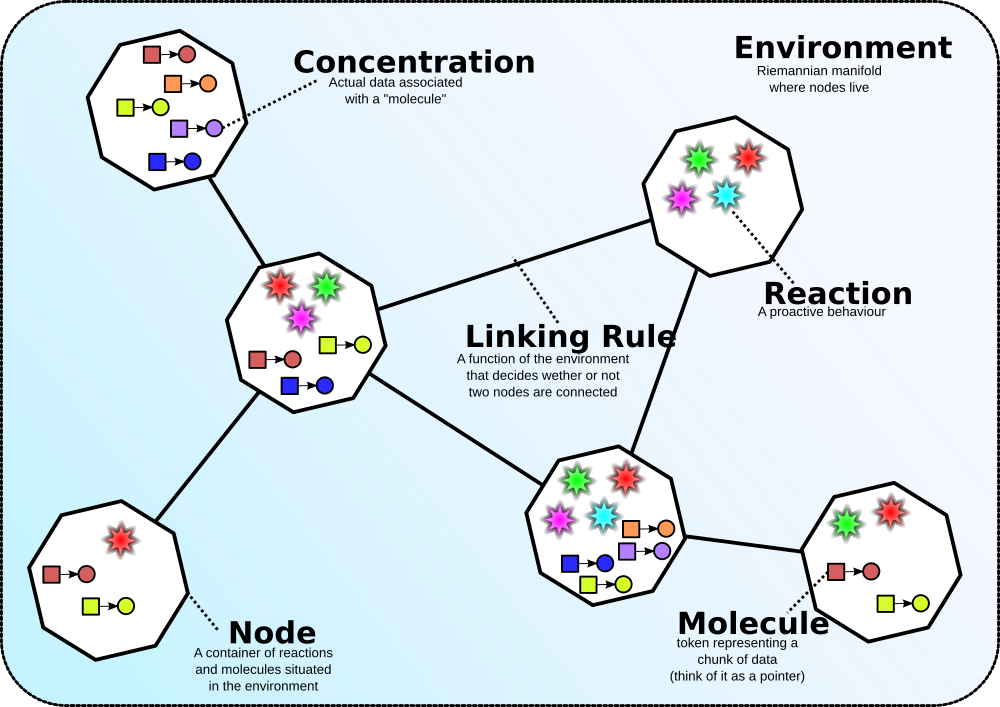
\includegraphics[width=12.5cm]{images/model.png} % inserisce una figura larga 12.5cm
% inserisce la legenda ed etichetta la figura con \label{fig:prima}
\caption[Illustrazione meta-modello di Alchemist]{Illustrazione meta-modello di Alchemist} \label{fig:alchemistModel}
\end{center}
\end{figure}

L'\textbf{\textit{Environment}} \`e l'astrazione dello spazio ed \`e anche l'entit\`a pi\`u esterna che funge da contenitore per i nodi. Conosce la posizione di ogni nodo nello spazio ed \`e quindi in grado di fornire la distanza tra due di essi e ne permette inoltre lo spostamento.

\`E detta \textbf{\textit{Linking rule}} una funzione dello stato corrente dell'environemnt che associa ad ogni nodo un \textbf{\textit{Vicinato}}, il quale \`e un entit\`a composta da un nodo centrale e da un set di nodi vicini.

Un \textbf{\textit{Nodo}} \`e un contenitore di molecole e reazioni che \`e posizionato all'interno di un environment.

La \textbf{\textit{Molecola}} \`e il nome di un dato, paragonabile a quello che rappresenta il nome di una variabile per i linguaggi imperativi.
Il valore da associare ad una molecola \`e detto \textbf{\textit{Concentrazione}}.

%crea l'ambiente figura;
\begin{figure}[h] % [h] sta per here, cioè la figura va qui
\begin{center} % centra nel mezzo della pagina la figura
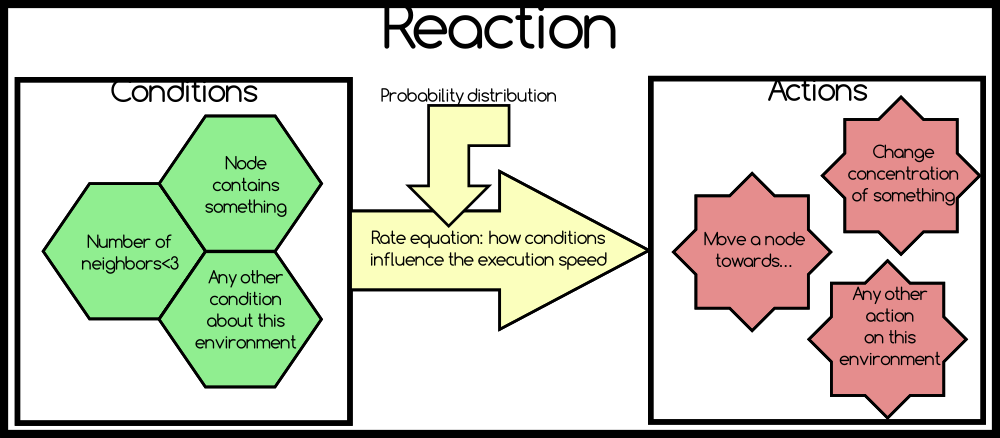
\includegraphics[width=14cm]{images/reaction.png} % inserisce una figura larga 12.5cm
% inserisce la legenda ed etichetta la figura con \label{fig:prima}
\caption[Illustrazione modello reazione di Alchemist]{Illustrazione modello reazione di Alchemist} \label{fig:alchemistReaction}
\end{center}
\end{figure}

Una \textbf{\textit{Reazione}} \`e un qualsiasi evento che pu\`o cambiare lo stato dell'environment ed \`e definita tramite una distribuzione temporale, una lista di condizioni e una o pi\`u azioni.
\\La frequenza con cui avvengono dipende da:
\begin{itemize}
\item un parametro statico di frequenza;
\item il valore di ogni condizione;
\item un'equazione di frequenza che combina il parametro statico e il valore delle condizioni restituendo la frequenza istantanea;
\item una distribuzione temporale.
\end{itemize}
Ogni nodo contiene un set di reazioni che pu\`o essere anche vuoto.

Per comprendere meglio il meccanismo di una reazione si pu\`o osservare la figura \ref{fig:alchemistReaction}.

Una \textbf{\textit{Condizione}} \`e una funzione che prende come input l'environment corrente e restituisce come output un booleano e un numero. Se la condizione non si verifica, le azioni associate a quella reazione non saranno eseguite. In relazione a parametri di configurazione e alla distribuzione temporale, una condizione potrebbe influire sulla velocit\`a della reazione.

La \textbf{\textit{Distribuzione temporale}} indica il numero di eventi che si verificano successivamente ed indipendentemente in un dato intervallo di tempo.

Un'\textbf{\textit{Azione}} \`e la definizione di una serie di operazioni che modellano un cambiamento nel nodo o nell'environment.

In Alchemist un'incarnazione \`e un'istanza concreta del meta-modello appena descritta e che implementa una serie di componenti base come: la definizione di una molecola e del tipo di dati della concentrazione, un set di condizioni, le azioni e le reazioni. Incarnazioni diverse possono modellare universi completamente differenti.

%++-++-++-++-++-++-++-++-++-++-++-++-++-++-++-++-++-++-++-++-++-++-++-++-++-++-
\section{Scrivere una simulazione}
% style for general source code
\lstset{
  numberstyle=\footnotesize\color{black},
  basicstyle=\ttfamily,
  breakatwhitespace=false,
  breaklines=true,
  captionpos=b,
  keepspaces=true,
  numbers=left,
  numbersep=0pt,
  showspaces=false,
  showstringspaces=false,
  showtabs=false,
  tabsize=2,
  frame=tb
  %label=incarnationYAML,
  %caption={First verbatim}
  %language=Java
  %escapeinside={(*@}{@*)}
}
Il linguaggio da utilizzare per scrivere le simulazioni in Alchemist \`e YAML e quello che il parser del simulatore si aspetta in input \`e una mappa YAML.
\\
Nei prossimi paragrafi verr\`a mostrato quali sezioni si possono inserire e come utilizzarle per creare la simulazione che si vuole realizzare.

La sezione \textbf{incarnation} \`e obbligatoria. Il parser YAML si aspetta una stringa che rappresenta il nome dell'incarnazione da utilizzare per la simulazione.
\medskip
\begin{lstlisting}[firstnumber=last,caption={Incarnazione}]
  incarnation: agent
\end{lstlisting}

Nel resto della sezione, il valore associato alla chiave 'type' fa riferimento al nome di una classe. Se il nome passato non \`e completo, ovvero non \`e comprensivo del percorso fino alla classe, Alchemist provveder\`a a cercare la classe tra i packages.

Per dichiarare variabili che poi potranno essere richiamate all'interno del file di configurazione della simulazione si pu\`o procedere in questo modo.
\medskip
\begin{lstlisting}[firstnumber=last,caption={Variabili simulazione}]
  variables:
    myVar: &myVar
      par1: 0
      par2: "string"
    mySecondVar: &myVar2
      par: "value"
\end{lstlisting}

Utilizzando la keyword \textbf{environment} si pu\`o scegliere quale definizione di ambiente utilizzare per la simulazione.
\medskip
\begin{lstlisting}[firstnumber=last,caption={Environment}]
  environment:
    type: OSMEnvironment
    parameters: [/maps/foo.pbf]
\end{lstlisting}
Questo parametro \`e opzionale e di default \`e uno spazio continuo bidimensionale: ometterlo equivale a scrivere la seguente configurazione.
\medskip
\begin{lstlisting}[firstnumber=last,caption={Default environment}]
  environment:
    type: Continuous2DEnvironment
\end{lstlisting}

La keyword \textbf{positions} consente di specificare il tipo delle coordinate della simulazione. La psizione riflette lo spazio fisico: per esempio non si potr\`a utilizzare la distanza \textit{Continuous2DEuclidean} se si considera la mappa di una citt\`a visto che dati due punti A e B, nel mondo reale la distanza AB \`e diversa da quella BA.
\medskip
\begin{lstlisting}[firstnumber=last,caption={Default environment}]
  positions:
    type: LatLongPosition
\end{lstlisting}

I collegamenti tra i nodi che verranno utilizzati nella simulazione sono specificati nella sezione \textbf{network-model}. Un esempio per la costruzione di collegamenti \`e il seguente.
\medskip
\begin{lstlisting}[firstnumber=last,caption={Funzione linking-rule}]
  network-model:
    type: EuclideanDistance
    parameters: [10]
\end{lstlisting}
Anche questo \`e un parametro opzionale e di default non ci sono collegamenti, ovvero i nodi nell'environemnt non sono collegati, ed \`e descritto con il seguente formalismo.
\medskip
\begin{lstlisting}[firstnumber=last,caption={Default linking-rule}]
  network-model:
    type: NoLinks
\end{lstlisting}

Il posizionamento dei nodi viene gestito dalla sezione \textbf{displacements}. Questa sezione pu\`o contenere uno o pi\`u definizioni di disposizioni per i nodi.
Il parametro 'in' definisce la geometria all'interno del quale verranno disposti i nodi, utilizzando ad esempio punti o figure come cerchi o rettangoli, mentre il parametro 'programs' definisce le reazioni da associare ad ogni nodo di quella certa disposizione.
\\
Esempi di classi utilizzabili nel parametro 'in' sono Point e Circle.
La classe Circle necessita di quattro parametri, da passare nel seguente ordine: il numero di nodi da disporre, la coordinata x del centro, la coordinata y del centro, il raggio del cerchio. Per la classe Point \`e sufficiente fornire in ordine la coordinata x e la coordinata y.

Il parametro 'programs' rappresenta le reazioni da associare ai nodi ed accetta una lista di reazioni, le quali a loro volta sono formate da una lista di parametri. Un'esempio di definizione di una reazione \`e utilizzando 'time-distribution' (valore utilizzato per settare la freqeunza) e 'program' (parametro che viene passato alla creazione della reazione e che pu\`o essere utilizzato per istanziare condizioni e azioni).
Un'esempio di displacements \`e il seguente.
\medskip
\begin{lstlisting}[firstnumber=last,caption={Disposizione nodi e reazioni associate}]
  displacements:
    - in: {type: Circle, parameters: [5,0,0,2]}
      programs:
      -
        - time-distribution: 1
          program: "reactionParam"
        - time-distribution: 2
          program: "doSomethingParam"
    - in: {type: Point, parameters: [1,1]}
      programs:
      -
        - time-distribution: 1
          program: "pointReactionParam"
\end{lstlisting}


%-%-%-%-%-%-%-%-%-%-%-%-%-%-%-%-%-%-%-%-%-%-%-%-%-%-%-%-%-%-%-%-%-%-%-%-%-%-%-%-
\chapter{Agenti}
% imposta l'intestazione di pagina
\lhead[\fancyplain{}{\bfseries\thepage}]{\fancyplain{}{\bfseries\rightmark}}

Un'agente \`e un entit\`a che agisce in modo autonomo e continuo in uno spazio condiviso con altri agenti. Le caratteristiche principali di un agente sono: autonomia, proattivit\`a e reattivit\`a. Gli agenti sono formati da un nome, che \`e una caratteristica statica, e da componenti dinamici come lo stato.

%++-++-++-++-++-++-++-++-++-++-++-++-++-++-++-++-++-++-++-++-++-++-++-++-++-++-
\section{Agenti BDI}
Gli agenti BDI forniscono un meccanismo per separare le attivit\`a di selezione di un piano fra quelli presenti nella sua teoria dall'esecuzione del piano attivo, permettendo di bilanciare il tempo speso nella scelta del piano e quello per eseguirlo.

I \textbf{\textit{Beliefs}} sono informazioni dello stato dell'agente, ovvero ci\`o che l'agente sa del mondo (di se stesso e degli altri agenti), e possono comprendere regole di inferenza per permettere l'aggiunta di nuovi beliefs. L'insieme dei beliefs di un agente \`e detto 'belief base' o 'belief set' e si pu\`o modificare nel tempo.

I \textbf{\textit{Desires}} sono tutti i possibili piani che l'agente potrebbe eseguire. Rappresentano gli obiettivi o le situazioni che l'agente vorrebbe realizzare o portare a termine. I \textbf{goals} sono desires che l'agente persegue attivamente: per questo motivo, in generale, i piani desiderabili possono non essere coerenti tra loro mentre i goals \`e bene che lo siano.

Le \textbf{\textit{Intentions}} sono piani a cui l'agente ha deciso di lavorare o a cui sta gi\`a lavorando. I piani sono sequenze di azioni che un agente pu\`o eseguire per raggiungere una intention. I piani possono contenerne altri al loro interno.

Gli \textbf{\textit{Eventi}} innescano le attivit\`a reattive degli agenti il cui risultato pu\`o essere l'aggiornamento dei beliefs, la chiamata ad altri piani o la modifica di goals.

%++-++-++-++-++-++-++-++-++-++-++-++-++-++-++-++-++-++-++-++-++-++-++-++-++-++-
\section{tuProlog}
tuProlog \`e un interprete Prolog per le applicazioni e le infrastrutture Internet basato su Java. \`E progettato per essere facilmente utilizzabile, leggero, configurabile dinamicamente, direttamente integrato in Java e facilmente interoperabile.

tuProlog \`e sviluppato e mantenuto da 'aliCE' un gruppo di ricerca dell'Alma Mater Studiorum - Universit\`a di Bologna, sede di Cesena. \`E un software Open Source e rilasciato sotto licenza LGPL.

Il motore tuProlog fornisce e riconosce i seguenti tipi di predicati:
\begin{itemize}
  \item predicati built-in: incapsulati nel motore tuProlog.
  \item predicati di libreria: inseriti in una libreria che viene caricata nel motore tuProlog. La libreria pu\`o essere liberamente aggiunta all'inizio o rimossa dinamicamente durante l'esecuzione. I predicati della libreria possono essere sovrascritti da quelli della teoria. Per rimuovere un singolo predicato dal motore \`e necesssario rimuovere tutta la libreria che contiene quel predicato.
  \item predicati della teoria: inseriti in una teoria che viene caricata nel motore tuProlog. Le teorie tuProlog sono semplicemente collezioni di clausole Prolog. Le teorie possono essere liberamente aggiunte all'inizio o rimosse dinamicamente durante l'esecuzione.
\end{itemize}

Librerie e teorie, pur essendo simili, sono gestite diversamente dal motore tuProlog.

\chapter{Spatial Tuples}
Spatial Tuples \`e un'estensione del modello base di tuple per i sistemi distribuiti multi agente dove:
\begin{itemize}
   \item le tuple sono posizionate nel mondo fisico e si possono muovere;
   \item il comportamento delle primitive di coordinamento pu\`o dipendere dalla propriet\`a spaziali del coordinamento degli agenti;
   \item lo spazio di tuple pu\`o essere concepito come un livello virtuale che aumenta la realt\`a fisica.
\end{itemize}

Questo modello supporta la consapevolezza dello spazio e la coordinazione basata sullo spazio dell'agente in scenari di calcolo pervasivo.

\section{Tuple spaces}
Uno spazio di tuple \`e un implementazione del paradigma di memoria associativa per l'elaborazione parallela/distribuita. Fornisce un repository di tuple al quale \`e possibile accedere contemporaneamente. Lo spazio di tuple pu\`o essere considerato come una forma di memoria condivisa distribuita. Ci sono due categorie di utilizzatori dello spazio di memoria: chi scrive e chi legge. I primi aggiungono tuple allo spazio di memoria condiviso mentre i secondi rimuovono quelle che corrispondono ad un determinato template.

\section{Modello Spatial Tuples}\label{ModelloSpatialTuples}
In questa estensione le informazioni hanno una posizione e una estensione nello spazio fisico: lo spazio di tuple \`e quindi concepito come un aumento della realt\`a fisica dove le tuple rappresentano uno strato di informazioni associate ad un'informazione spaziale.
Una volta che la tupla \`e associata ad una regione o posizione, le informazioni sono propriet\`a che possono essere attribuite a quella porzione di spazio fisico.

Le primitive che permettono la comunicazione sono:
\begin{itemize}
   \item out(t): emette tuple spaziali t e le associa ad una regione
   \item rd(tt): ricerca tuple che corrispondano al template tt e le ritorna
   \item in(tt): ricerca tuple che corrispondano al template tt e le consuma
\end{itemize}

Le richieste in Spatial Tuples sono sospensive e non deterministiche. Sospensive perch\`e se non ci sono tuple che fanno match con il template l'operazione \`e bloccata finch\`e non viene trovata la tupla. Il non determinismo, invece, deriva dal fatto che se ci fossero pi\`u tuple che corrispondono al template ne viene scelta una casualmente.

Le tuple spaziali possono essere associate a posizioni o regioni in modo diretto o indiretto. Le operazioni dirette associano direttamente la tupla spaziale ad una posizione o una regione. Quelle indirette, invece, associano tuple a componenti situati e vale anche se la regione in cui si trova il componente cambia nel tempo: finch\`e non viene rimossa, la tupla \`e associata alla regione del componente in cui \`e situata.

Spatial Tuples pu\`o essere utile nei domini applicativi in cui la reatl\`a \`e aumentata o mista, ovvero in scenari in cui gli esseri umani si spostano all'interno di un ambiente fisico aumentato e devono coordinarsi con altri utenti o agenti di qualsiati tipo (situati o non situati).

%-%-%-%-%-%-%-%-%-%-%-%-%-%-%-%-%-%-%-%-%-%-%-%-%-%-%-%-%-%-%-%-%-%-%-%-%-%-%-%-
\chapter{Progetto}
% imposta l'intestazione di pagina
\lhead[\fancyplain{}{\bfseries\thepage}]{\fancyplain{}{\bfseries\rightmark}}

Il progetto, come descritto nell'introduzione, ha come obiettivo l'implementazione del meta-modello di Alchemist attraverso la definizione di un incarnazione che modelli Spatial Tuples attraverso gli agenti all'interno del simulatore.

Per la realizzazione del ciclo di ragionamento dell'utente si \`e utilizzato il motore tuProlog importato e invocato all'interno del simulatore sfruttando la libreria 'aliCE'.

%++-++-++-++-++-++-++-++-++-++-++-++-++-++-++-++-++-++-++-++-++-++-++-++-++-++-
\section{Mapping dei modelli}
Il primo passo nell'evoluzione del progetto \`e stata l'analisi del mapping tra il meta-modello di Alchemist e il modello ad agenti, necessaria per individuare eventuali incongruenze o evidenziare opportunit\`a a livello applicativo e maggiore espressivit\`a.
Nei mapping effettuati si \`e cercato quindi di individuare l'entit\`a del meta-modello di Alchemist che offrisse maggiori opportunit\`a espressive per la definizione dell'agente.

Nella prima prova, l'agente \`e stato riferito ad un nodo, da cui ne deriva che l'environment sar\`a lo spazio che conterr\`a tutti gli agenti. Internamente al nodo, le molecole e le concentrazioni saranno utilizzate per gestire i beliefs dell'agente e le reazioni che saranno riferite ai piani utilizzando le condizioni come clausola per far scattare le azioni.
\\
Questo tipo di mapping consente di realizzare simulazioni di sistemi non complessi in cui vi \`e un solo 'livello' di agenti che interagiscono tra loro. Questa affermazione pu\`o essere compresa meglio analizzando il secondo tentativo che \`e stato effettuato.

Nel secondo mapping, l'agente \`e stato spostato pi\`u internamente al nodo riferendolo ad una reazione facendo diventare il nodo stesso uno spazio per gli agenti. In questo modo l'environment sar\`a uno spazio in cui possono essere presenti pi\`u nodi, i quali a loro volta potranno contenere un set di agenti.
\\
Utilizzando questo secondo caso si riuscir\`a a creare un sistema con pi\`u agenti all'interno di un singolo nodo, che in ambito applicativo pu\`o essere riferito ad un device, il quale si muover\`a nello spazio insieme ad altri nodi, contenitori di altri agenti.

La frequenza con cui gli eventi di Alchemist sono innescati dipende, oltre che dai parametri passati nella configurazione della simulazione, anche dalle condizioni definite per quello specifico agente: questo influisce sul numero di volte in cui viene eseguita un'azione.

\section{Definizione del linguaggio}
Dopo aver effettuato l'analisi dei vari mapping si \`e passati alla realizzazione di un linguaggio per l'incarnazione. Lo scopo di questa operazione \`e quella di fornire all'utilizzatore finale, ovvero il programmatore dell'agente, completa libert\`a per la definizione della teoria dell'agente ma che al tempo stesso permetta di gestire il comportamento dell'agente all'interno dell'ambiente di simulazione.

Per programmare l'agente sono messi a disposizione i seguenti beliefs:
\begin{itemize}
   \item \textbf{self(A).} Rappresenta il nome dell'agente riferito dal termine A
   \item \textbf{belief(position(X,Y)).} Memorizza nell'agente le coordinate della posizone del nodo che lo ospita
   \item \textbf{belief(movement(S,D)).} Mantiene le informazioni relative a velocit\`a (S) e direzione (D), rappresentata come angolo in radianti, del nodo in cui \`e posizionato l'agente
   \item \textbf{belief(distance(A,D)).} Ogni agente ha al suo interno N-1 di questi beliefs dove N \`e il numero totale degli agenti; rappresenta la distanza (D) di ogni agente del vicinato (A): il vicinato \`e calcolato con la linking-rule definita nella configurazione della simulazione
\end{itemize}

Per quanto riguarda i piani disponibili vi sono due tipologie: quelli che innescano un evento e quelli invocati per reagire ad un evento.
I piani che fanno parte del primo tipo sono:
\begin{itemize}
   \item \textbf{addBelief(B).} Aggiunge un belief alla 'belief base'
   \item \textbf{removeBelief(B).} Rimuove un belief dalla 'belief base'.
\end{itemize}
L'altra tipologia riguarda piani invocati per consentire all'agente di reagire ad un evento. Il comportamento degli agenti dipende dall'implementazione del corpo del piano definita dal programmatore dell'agente. Nella teoria dell'agente \`e possibile definire pi\`u piani per ognuna delle seguenti tipologie: solo per 'init' \`e possibile definire una sola implementazione.
\begin{itemize}
   \item \textbf{init.} Invocato all'inizializzazione dell'agente cio\`e la prima volta che viene eseguito il ciclo di ragionamento
   \item \textbf{onAddBelief(B).} Ad ogni inserimento di nuovi belief o aggiornamento della 'belief base' (come quello per la posizione o la distanza dagli altri agenti) viene invocato questo piano passando come termine il belief
   \item \textbf{onRemoveBelief(B).} Richiamato ad ogni rimozione di belief dalla 'belief base'
\end{itemize}

Per inserire il modello Spatial Tuples all'interno dell'incarnazione,sono state analizzate le sue parti per decidere l'implementazione delle primitive da fornire al programmatore dell'agente, permettergli di far comunicare gli agenti con gli spazi di tuple. Sono stati quindi definiti i piani che rispecchiano le primitive \textbf{out(t)}, \textbf{rd(tt)}, \textbf{in(tt)} definte dal modello Spaital Tuples e un piano per la ricezione delle tuple prelevate. Mentre i primi tre sono piani che innescano un'azione, il quarto \`e un piano invocato per reagire alle operazioni di \textit{read} e \textit{write} e che il programmatore dell'agente sceglie come implementare.

\begin{itemize}
   \item \textbf{writeTuple(T).} Scrive una tupla T nello spazio di tuple pi\`u vicino.
   \item \textbf{readTuple(TT).} Cerca negli spazi di tuple del suo vicinato una tupla che corrisponda al template TT.
   \item \textbf{takeTuple(TT)}. Stessa procedura di readTuple ma se la tuple viene trovata \`e rimossa dallo spazio di tuple.
   \item \textbf{onResponseMessage(T).} Piano invocato dal sistema in cui viene passata la tupla recuperata con gli eventi scatenati da readTuple e writeTuple.
\end{itemize}

Le implementazioni dei piani che scatenatno un evento (mostrata nel Codice sorgente \ref{lst:LibreriaAgenti}) sono racchiuse all'interno della libreria caricata nel motore tuProlog di ogni agente.

\medskip
\begin{lstlisting}[firstnumber=1,label={lst:LibreriaAgenti},caption={Libreria agenti}]
   addBelief(B) :-
     assertz(belief(B)),
     assertz(added_belief(B)).

   removeBelief(B) :-
     retract(belief(B)),
     assertz(removed_belief(B)).

  writeTuple(T) :-
     assertz(write(T)).

  readTuple(TT) :-
     assertz(read(TT)).

  takeTuple(TT) :-
     assertz(take(TT)).
\end{lstlisting}

\section{Definizione incarnazione}
Lo sviluppo dell'incarmazione \`e partito dalla definizione della classe \textbf{AgentIncarnation} che implementa l'interfaccia \textit{Incarnation}. I metodi definiti nell'interfaccia consentono di caratterizzare l'incarnazione nella creazione delle varie entit\`a del modello (nodi, distribuzioni temporali, reazioni, condizioni, azioni).

Per la creazione del \textbf{nodo} si \`e definita la classe \textbf{AgentsContainerNode} che estende \textit{AbstractNode}. Questa classe ha tra le sue propriet\`a il riferiemnto all'environment in cui si trova il nodo, una struttura dati composta da coppie chiave e valore (in cui la chiave \`e il nome dell'agente e il valore \`e il riferimento all'azione dell'agente) e valori di velocit\`a e direzione per lo spostamento.

La \textbf{distribuzione temporale} di ogni reazione \`e stata realizzata istanziando la classe \textit{DiracComb} inizializzata con il parametro recuperato dal file di configurazione della simulazione. La classe permette di emettere eventi ad un intervallo temporale specificato dal parametro passato.

Per le \textbf{reazioni} \`e stata definita la classe \textbf{AgentReaction} che implementa \textit{AbstractReaction} e che rappresenta l'agente e che contiene le azioni, che sono il fulcro dell'agente, e le condizioni che devono verificarsi per far avvenire le azioni. Come propriet\`a della classe \`e presente solo una stringa che memorizza il nome dell'agente.
\\
La creazione delle \textbf{condizioni} \`e stata definita istanziando la classe \textit{AbstractCondition} e implementando i metodi mancanti dell'interfaccia Condition: \textit{getContext} (definisce la profondit\`a della condizione tra GLOBAL, NEIGHBORHOOD, LOCAL), \textit{getPropensityContribution} (permette di influenzare la velocit\`a della reazione che decide se utilizzare o meno questo parametro), \textit{isValid} (definisce la clausola per la valit\`a della condizione).
\\
L'\textbf{azione} da creare \`e passata dalla reazione tramite un parametro. Nell'azione verr\`a gestito il ciclo di ragionamento dell'agente con il metodo \textit{execute} definito nell'interfaccia \textit{Action} e saranno utilizzati i costrutti forniti dalla libreria 'alice.tuprolog' per invocare i piani della teoria dell'agente e poi gestirne il risutlato in Alchemist.

Per le azioni si \`e voluto creare una struttura con una classe principale che implementa i metodi per gestire il comportamento degli agenti e che sia estesa da altre classi, le quali implementino il ciclo di ragionamento invocando i metodi della classe padre

Seguendo questa logica \`e stata creata la classe astratta \textbf{AbstracAgent} che estende \textit{AbstractAction} e che, dei metodi rimasti da implementare dell'interfaccia \textit{Action}, definisce solamente \textit{getContext} lasciando alla classe dell'agente che si vuole creare la capacit\`a di implementare \textit{execute} e \textit{cloneAction}, rispettivamente utilizzati per il ciclo di ragionamento e per clonare l'azione.
Nella classe astratta creata, sono state quindi definite le variabili per la gestione dell'agente, tra cui quelle per le code dei messaggi (entrata e uscita), il motore tuProlog e una struttura per la notifica dei cambiamenti della 'belief base'. Nel costruttore viene caricata inoltre la libreria definita nel Codice sorgente \ref{lst:LibreriaAgenti} nella quale sono descritti i piani che definiscono il linguaggio e invocabili nella teoria dell'agente.
\\
La classe inoltre contiene i metodi per il comportamento dell'agente nel ciclo di ragionamento e quelli per l'inizializzazione. Quest'ultima \`e identificata come la prima esecuzione del ciclo di ragionamento dell'agente e che quindi racchiude delle istruzioni basilari per la sua corretta operativit\`a.

Estendendo la classe appena descritta \`e stata creata \textbf{SimpleAgent} che racchiude tutte le caratteristiche principali di un agente descritte precedentememte. Alla sua istanziazione, oltre a richiamare il costruttore del padre, carica nel motore tuProlog il file contenente la sua teoria. Gli unici metodi rimasti da definire per creare l'agente sono \textit{execute} e \textit{cloneAction}.
L'implementazione del primo \`e mostrata \ref{lst:SimpleAgentReasoningCycle} mentre la seconda \`e semplicemente la creazione di una nuova istanza dell'oggetto che prende il nome 'cloned\_' seguito dal nome dell'agente (es. per l'agente 'bob' verr\`a creato l'agente 'cloned\_bob').

\medskip
\begin{lstlisting}[firstnumber=1,label={lst:SimpleAgentReasoningCycle},caption={Simple Agent Reasoning Cycle}]
   if (!this.isInitialized()) {
      //Agent's first reasoning cycle
      this.inizializeAgent();

      this.initReasoning();
   } else {
      //Agent's reasoning cycle

      this.positionUpdate();

      this.getBeliefBaseChanges();

      this.notifyBeliefBaseChanges();
   }
\end{lstlisting}

Se l'agente non \`e inizializzato vengono invocati in sequenza i metodi \textit{inizializeAgent} e \textit{initReasoning}. Il primo inizializza l'agente, impostando nella teoria alcuni belief  tra cui quello per la posizione e per lo spostamento del nodo. Il secondo invece effettua la chiamata al piano 'init' eseguendo la configurazione iniziale definita dal programmatore dell'agente.

Il metodo \textbf{\textit{positionUpdate}}, riguarda l'aggiornamento della posizione. Per prima cosa viene calcolata la nuova posizione, poi rimossa la precedente dalla teoria dell'agente e quindi inserita quella nuova. L'aggiornamento della posizione produce due azioni: la preparazione per la notifica dell'evento di aggiornamento e la chiamata al metodo \textit{getNeighborhoodDistances}. La prima avviene aggiungendo il belief nella mappa delle notifiche dei cambiamenti della 'belief base' mentre la seconda prevede il calcolo della distanza di ogni agente da quello agente corrente: questa seconda azione opera l'aggiornamento dei belief e quindi una modifica della 'belief base', che comporta l'aggiunta dei belief alla mappa per la notifica degli eventi.

Il metodo \textbf{\textit{getBeliefBaseChanges}} recupera dalla teoria dell'agente i belief del tipo 'added\_belief(B)' o 'removed\_belief(B)', ovvero quelli aggiunti da chiamate ai piani 'addBelief(B)' o 'removeBelief(B)'. Per ogni belief aggiunto o rimosso lo aggiunge alla mappa per la notifica degli eventi.

Nel metodo \textbf{\textit{notifyBeliefBaseChanges}} viene presa la mappa con tutti i belief aggiunti in precedenza e per ogni belief viene invocato il piano 'onAddBelief(B)' o 'onRemoveBelief(B)' a seconda che il piano sia stato rispettivamente aggiunto o rimosso dalla 'belief base'. Nel caso della posizione e della distanza tra gli agenti, per gestire l'aggiornamento, viene inserito, e quindi notificato, solamente il belief di aggiunta.


\subsection{Spostamento del nodo}
Per realizzare lo spostamento sono stati utilizzati i campi per memorizzare la velocit\`a di spostamento del nodo, la direzione o angolo dello spostamento (rappresentata da un valore espresso in radianti) e il tempo della simulazione in cui \`e avvenuto l'ultimo aggiornamento della posizione della classe AgentsContainerNode.
Oltre a queste propriet\`a sono presenti anche i metodi per recuperare e aggiornare tali valori.
\\
Il metodo che effettua lo spostamento vero e proprio del nodo \`e \textit{changeNodePosition} che prende come parametro il tempo della simulazione corrente e ad ogni ciclo ci ragionamento effettua l'aggiornamento della posizone del nodo che ospita l'agente. L'implementazione del metodo \`e mostrata nel Codice sorgente \ref{lst:changeNodePosition}. All'interno del metodo viene costruito un cerchio che ha come centro le coordinate attuali del nodo e come raggio la differenza di tempo rispetto al precedente spostamento moltiplicata per la velocit\`a. La nuova posizione \`e un punto della circonferenza che viene individuato utilizzando l'angolo o direzione del nodo.
\medskip
\lstset{
  numberstyle=\footnotesize\color{black},
  basicstyle=\ttfamily,
  breakatwhitespace=true,
  breaklines=true,
  captionpos=b,
  keepspaces=true,
  numbers=left,
  numbersep=0pt,
  showspaces=false,
  showstringspaces=false,
  showtabs=false,
  tabsize=2,
  frame=tb,
  language=Java,
  commentstyle=\color{gray},
  keywordstyle=\color{blue},
  stringstyle=\color{red}
}
\begin{lstlisting}[firstnumber=1,label={lst:changeNodePosition},caption={Implementazione spostamento nodo}]
public void changeNodePosition(final Time time) {
  final Position currPos = this.getNodePosition();
  final double radAngle =  this.nodeDirectionAngle;

  // radius = space covered = time spent * speed
  final double radius = (time.toDouble() - this.lastUpdataTime.toDouble()) * this.nodeSpeed;

  final double x = currPos.getCoordinate(0) + radius * Math.cos(radAngle);

  final double y = currPos.getCoordinate(1) + radius * Math.sin(radAngle);

  this.environment.moveNodeToPosition(
     this, this.environment.makePosition(x, y));

  this.lastUpdataTime = time;
 }
\end{lstlisting}

\subsection{Aggiornamento belief base}
Per quanto riguarda l'aggiornamento delle 'belief base' si \`e pensato di incapsulare i predicati 'asserta', 'assertz' e 'retract' utilizzando strutture dati e piani tuPorlog per svolgere lo stesso comportamento: modifica della 'belief base', notifica del cambiamento tramite evento. In questo modo si \`e in grado di spezzare l'inserimento o la rimozione del belief dalla notifica del cambiamento, evitando che un agente operi un ciclo di ragionamento senza mai terminare, ovvero che l'agente continui a svolgere compiti lato tuProlog senza far tornare il controllo delle ad Alchemist.
\\
La prima parte, quella dell'aggiunta o rimozione del belief dalla 'belief base', \`e incapsulata all'interno dei piani 'addBelief(B)' e 'removeBelief(B)' i quali inoltre si occupano di aggiungere un'altro belief fittizio ('added\_belief(B)' o 'removed\_belief(B)') che verr\`a utilizzato per divulgare l'evento.
La parte di notifica viene svolta da Alchemist ed \`e divisa in due fasi: inizialmente viene recuperato il belief fittizio e inserito il suo termine all'interno di una mappa, dopodich\`e quest'ultima viene iterata e per ogni belief viene invocato un evento 'onAddBelief(B)' o 'onRemoveBelief(B)' relativamente alla tipologia di modifica della 'belief base' avvenuta e dove il B \`e il termine recuperato precedentemente.
La definizione dei piani per aggiungere e rimuovere i belief \`e la seguente.
\medskip
\lstset{
  numberstyle=\footnotesize\color{black},
  basicstyle=\ttfamily,
  breakatwhitespace=false,
  breaklines=true,
  captionpos=b,
  keepspaces=true,
  numbers=left,
  numbersep=0pt,
  showspaces=false,
  showstringspaces=false,
  showtabs=false,
  tabsize=2,
  frame=tb,
  commentstyle=\color{black},
  keywordstyle=\color{black},
  stringstyle=\color{black}
  %label=incarnationYAML,
  %caption={First verbatim}
  %language=Java
  %escapeinside={(*@}{@*)}
}
\begin{lstlisting}[firstnumber=1,caption={Implementazione piani per l'aggiunta e rimozione di belief}]
   addBelief(B) :-
     assertz(belief(B)),
     assertz(added_belief(B)).

   removeBelief(B) :-
     retract(belief(B)),
     assertz(removed_belief(B)).
\end{lstlisting}

%-%-%-%-%-%-%-%-%-%-%-%-%-%-%-%-%-%-%-%-%-%-%-%-%-%-%-%-%-%-%-%-%-%-%-%-%-%-%-%-
\subsection{Implementazione Spatial Tuples}
Per modellare le posizioni degli spazi di tuple, \`e stata definita la classe \textbf{Blackboard} che estende da \textbf{AbstractAgent} e implementa una specializzazione dell'agente. Questa classe rappresenta un punto situato nello spazio che pu\`o contenere informazioni: gli agenti possono, attraverso le primitive descritte nel Codice sorgente \ref{lst:LibreriaAgenti}, scrivere tuple oppure leggere o prendere quelle che corrispondono al template passato.
All'interno della classe sono state create due liste una per le richieste in entrata e una per quelle in attesa. La classe espone il metodo \textit{insertRequest} al quale sono passati la tupla/template, l'istanza dell'agente e l'azione da eseguire (\textit{write}/\textit{read}/\textit{take}). La richiesta viene aggiunta alla coda e processata nel ciclo di ragionamento dell'istanza di questo agente. In base alla tipologia di azione vengono invocati i diversi metodi interni \textit{writeOnBlackboard}, \textit{readOnBlackboard}, \textit{takeOnBlackboard} per la gestioni della richiesta.
Come detto nella sezione \ref{ModelloSpatialTuples}, se le operazioni richieste non possono essere effettuate vengono sospese e inserite nella coda di quelle in attesa: questa lista viene iterata, come quella delle richieste in entrata, ad ogni ciclo di ragionamento.
\\
Per le richieste di tipo \textit{read} e \textit{take}, se l'operazione di match del template va a successo deve essere notificata all'agente la tupla letta/prelevata. Questa azione \`e fatta inserendo nella struttura di notifica dei belif dell'agente un nuovo elemento, che \`e la tupla recuperata dallo spazio di tuple, e che verr\`a notificata nel prossimo ciclo di ragionamento dell'agente.

Per completare l'implementazione di Spatial Tuples \`e necessario definire un metodo nella classe AbstracAgent che consente agli agenti, durante il loro ciclo di ragionamento, di recuperare i beliefs inseriti con i piani descritti nel Codice sorgente \ref{lst:LibreriaAgenti} e di inserirli nello spazio di tuple. \`E stato quindi implementato il metodo \textit{retrieveTuples} che per prima cosa recupera tutte le tuple dalla teoria dell'agente e poi in base al tipo di azione esegue delle operazioni diverse.
\\
Se l'azione \`e \textit{write}, cerca l'agente di tipo Blackboard pi\`u vicino e se lo trova invoca il metodo per inserire la richiesta.
\\
Diversamente, se l'azione \`e \textit{read} o \textit{take}, viene recuperata la lista di agenti di tipo Blackboard presenti nel suo vicinato. Per ognuno degli agenti della lista viene inserita la richiesta in modo tale da estendere la ricerca della tupla che corrisponda al template.

\section{Simulazione}
Per testare l'incarnazione creata \`e stato utilizzato il pattern di coordinazione 'breadcrumbs'. L'esempio prodotto utilizza due agenti, Hansel e Gretel, che si muovono all'interno di un'ambiente in cui sono presenti altri agenti utilizzati come spazi di tuple situati. L'agente Hansel si sposter\`a casualmente nell'ambiente lasciando le briciole negli spazi di tuple pi\`u vicini al suo passaggio, mentre l'agente Gretel dovr\`a muoversi alla ricerca delle briciole e una volta che ne ha individuata una iniziare a seguire le altre per raggiungere Hansel.

Per realizzare questa simulazione \`e stato scritto il file di configurazione indicato dal Codice sorgente \ref{lst:SimulazioneBreadcrumbs}.
\medskip
\begin{lstlisting}[firstnumber=1,label={lst:SimulazioneBreadcrumbs},caption={Simulazione modello Spatial Tuples con modello di coordinazione breadcrumbs}]
   incarnation: agent

   network-model:
   type: ConnectWithinDistance
   parameters: [0.5]

   displacements:
   - in: {type: Circle, parameters: [1,-1.8,2,0.2]}
   programs:
      -
        - time-distribution: 1
          program: "hansel"

   - in: {type: Circle, parameters: [1,2,2,0.2]}
   programs:
      -
        - time-distribution: 1
          program: "gretel"

   - in: {type: Circle, parameters: [1000,2,2,4.5]}
   programs:
      -
        - time-distribution: 1
          program: "blackboard"
\end{lstlisting}

Le teorie degli agenti utilizzate in questa simulazione sono indicate qui di seguito.

\medskip
\begin{lstlisting}[firstnumber=1,label={lst:Hansel},caption={Teoria agente Hansel}]
   init :-
       writeTuple(breadcrumb(hansel,here)),
       removeBelief(movement(S,D)),
       addBelief(movement(0.025,4.8)),
       addBelief(counter(0,0)),
       addBelief(spiralCorner(0.08)),
       addBelief(stopped(false)).

   onAddBelief(position(X,Y)) :-
       belief(stopped(false)),
       removeBelief(counter(C1,C2)),
       handlePosition(C1,C2,X,Y).

   onAddBelief(position(X,Y)) :-
       true.

   handlePosition(C1,C2,X,Y) :-
       C1 < 300,
       C2 < 10,
       C1N is C1 + 1,
       C2N is C2 + 1,
       addBelief(counter(C1N,C2N)),
       writeTuple(breadcrumb(hansel,here)).

   handlePosition(C1,C2,X,Y) :-
       C1 < 300,
       C1N is C1 + 1,
       C2 >= 10,
       addBelief(counter(C1N,0)),
       removeBelief(movement(S,D)),
       belief(spiralCorner(V)),
       D1 is D + V,
       addBelief(movement(S,D1)).

   handlePosition(C1,C2,X,Y) :-
       C1 >= 300,
       C2N is C2 + 1,
       addBelief(counter(0,C2N)),
       removeBelief(spiralCorner(V)),
       TEMP is V * 0.30,
       V1 is V + TEMP,
       addBelief(spiralCorner(V1)).

   onAddBelief(distance(A,ND,OD)) :-
       true.

   onAddBelief(distance(gretel,ND)) :-
       removeBelief(stopped(false)),
       addBelief(stopped(true)),
       removeBelief(movement(_,D)),
       addBelief(movement(0,D)).

   onAddBelief(distance(A,ND)) :-
       true.

   onAddBelief(movement(_,_)) :-
       true.

   onRemoveBelief(movement(_,_)) :-
       true.

   onAddBelief(counter(C1,C2)) :-
       true.

   onRemoveBelief(counter(C1,C2)) :-
       true.

   onAddBelief(spiralCorner(V)) :-
       true.

   onRemoveBelief(spiralCorner(V)) :-
       true.

   onResponseMessage(msg(stop(hansel),X,Y)) :-
       removeBelief(movement(_,D)),
       addBelief(movement(0,D)),
       writeTuple(stop(gretel)).
\end{lstlisting}

\medskip
\begin{lstlisting}[firstnumber=1,label={lst:Gretel},caption={Teoria agente Gretel}]
   init :-
       removeBelief(movement(_,_)),
       randomDirection(D),
       addBelief(movement(0.025,D)),
       takeTuple(breadcrumb(hansel,here)),
       randomSteps(P),
       addBelief(counterStep(P)),
       addBelief(stopped(false)).

   onAddBelief(position(X,Y)) :-
       belief(stopped(false)),
       removeBelief(counterStep(S)),
       handlePosition(S,X,Y),
       takeTuple(breadcrumb(hansel,here)).

   onAddBelief(position(X,Y)) :-
       true.

   handlePosition(S,X,Y) :-
       S > 0,
       S1 is S - 1,
       addBelief(counterStep(S1)).

   handlePosition(S,X,Y) :-
       S =< 0,
       randomSteps(P),
       addBelief(counterStep(P)),
       removeBelief(movement(_,D)),
       randomDirection(RD),
       D1 is D - RD,
       addBelief(movement(0.025,D1)).

   onAddBelief(distance(hansel,ND,OD)) :-
       ND < 0.4,
       removeBelief(stopped(false)),
       addBelief(stopped(true)),
       removeBelief(movement(_,D)),
       addBelief(movement(0,D)).

   onAddBelief(distance(A,ND,OD)) :-
       true.

   onAddBelief(distance(A,ND)) :-
       true.

   onAddBelief(movement(_,_)) :-
       true.

   onRemoveBelief(movement(_,_)) :-
       true.

   onAddBelief(counterStep(C)) :-
       true.

   onRemoveBelief(counterStep(C)) :-
       true.

   onResponseMessage(msg(breadcrumb(hansel,here),X,Y)) :-
       removeBelief(counterStep(_)),
       addBelief(counterStep(15)),
       removeBelief(movement(_,D)),
       addBelief(movement(0.05,D)),
       changeDirection(X,Y).

   changeDirection(X2,Y2) :-
       belief(position(X1,Y1)),
       DX is X2 - X1,
       DY is Y2 - Y1,
       calculateAtan(DY,DX,RAD),
       removeBelief(movement(S,D)),
       addBelief(movement(S,RAD)).

   calculateAtan(DY,DX,RAD) :-
       DX > 0,
       RAD is atan(DY / DX).

   calculateAtan(DY,DX,RAD) :-
       DX < 0,
       DY >= 0,
       TMP is atan(DY / DX),
       RAD is TMP + 3.14.

   calculateAtan(DY,DX,RAD) :-
       DX < 0,
       DY < 0,
       TMP is atan(DY / DX),
       RAD is TMP - 3.14.

   calculateAtan(DY,DX,RAD) :-
       DX == 0,
       DY > 0,
       RAD is 3.14 / 2.

   calculateAtan(DY,DX,RAD) :-
       DX == 0,
       DY < 0,
       RAD is -3.14 / 2.

   randomSteps(R) :-
       rand_int(50,R).

   randomDirection(R) :-
       rand_float(X),
       TMP is X * 3.14,
       R is TMP - 1.57.
\end{lstlisting}

\medskip
\begin{lstlisting}[firstnumber=1,label={lst:Blackboard},caption={Teoria per gli spazi di tuple}]
   init :-
       true.
\end{lstlisting}

L'agente Hansel nella ricerca dell'agente Gretel esegue il seguente algoritmo. L'esecuzione dell'algoritmo \`e ciclica.
\begin{itemize}
   \item[(1)] ho trovato l'agente Hansel?
   \item[(2)] si: imposto la velocit\`a a 0 e aggiungo il belief stopped
   \item[(3)] no: ho trovato una briciola?
   \begin{itemize}
      \item[(4)] si: resetto il contatore dei passi e seguo la direzione della briciola a velocit\`a 0.05
      \item[(5)] no: ho fatto N passi senza trovare una briciola?
      \begin{itemize}
         \item[(6)] si: resetto il contatore dei passi, imposto una nuova direzione random e la velocit\`a a 0.025
         \item[(7)] no: decremento il contatore dei passi
      \end{itemize}
   \end{itemize}
\end{itemize}

\subsection{Raccolta dei dati}
Per valutare il grado di successo della simulazione sono state effettuate analisi sui risultati delle simulazioni. Su dieci di simulazioni eseguite, con la configurazone del Codice sorgente \ref{lst:SimulazioneBreadcrumbs} e con le teorie dei due agenti descritte nei Codici sorgenti \ref{lst:Hansel} e \ref{lst:Gretel}, \`e risultato che l'agente Hansel ha raggiunto Gretel nove volte con un tempo medio di 545 tau (tempo della simulazione).


% \clearpage{\pagestyle{empty}\cleardoublepage} % vedere se serve
\begin{thebibliography}{90} % crea l'ambiente bibliografia
\rhead[\fancyplain{}{\bfseries \leftmark}]{\fancyplain{}{\bfseries \thepage}}
% \addcontentsline{toc}{chapter}{Bibliografia} % aggiunge la voce Bibliografia nell'indice

% provare anche questo comando:
\addcontentsline{toc}{chapter}{\numberline{}{Bibliografia}}
\bibitem{K1} alchemistsimulator.github.io
\bibitem{K2} Programming Multi-Agent Systems in AgentSpeak using Jason, (Rafael H. Bordini, Jomi Fred H\"{u}bner, Michael Wooldridge), Wiley, Interscience (2007)

% \bibitem{K3} Terzo oggetto bibliografia.
% \bibitem{K4} Quarto oggetto bibliografia.
\end{thebibliography}
\end{document}
